% coding:utf-8

% Ausführen in R: 
% Sweave("C:/Daten/Daniel/studium/git_repo/sem2/stoc/sw10/sw10_2.Rnw",encoding='UTF-8')

\section{Aufgabe 2}

\subsection{a}
\begin{Schunk}
\begin{Sinput}
> plot(0:70,dnorm(x=0:70,mean=32,sd=6),type='h')
> abline(v=26,col='green')
> abline(v=38,col='green')
\end{Sinput}
\end{Schunk}
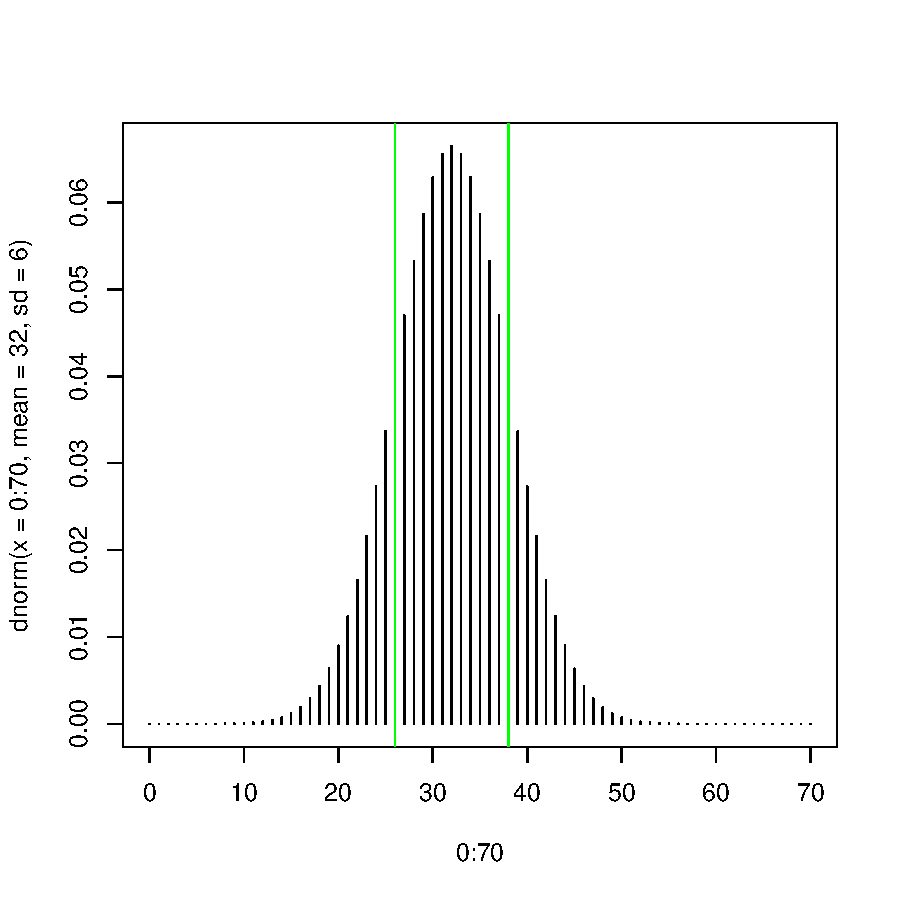
\includegraphics{sw10_2-001}

\subsection{b}
\begin{Schunk}
\begin{Sinput}
> pnorm(q=40,mean=32,sd=6)
\end{Sinput}
\begin{Soutput}
[1] 0.9087888
\end{Soutput}
\end{Schunk}

\subsection{c}
\begin{Schunk}
\begin{Sinput}
> pnorm(q=27,mean=32,sd=6)
\end{Sinput}
\begin{Soutput}
[1] 0.2023284
\end{Soutput}
\end{Schunk}

\subsection{d}
\begin{Schunk}
\begin{Sinput}
> qnorm(p=0.975,mean=32,sd=6)
\end{Sinput}
\begin{Soutput}
[1] 43.75978
\end{Soutput}
\end{Schunk}

\subsection{e}
\begin{Schunk}
\begin{Sinput}
> qnorm(p=0.1,mean=32,sd=6)
\end{Sinput}
\begin{Soutput}
[1] 24.31069
\end{Soutput}
\end{Schunk}

\subsection{f}
\begin{Schunk}
\begin{Sinput}
> pnorm(q=38,mean=32,sd=6)-pnorm(q=26,mean=32,sd=6)
\end{Sinput}
\begin{Soutput}
[1] 0.6826895
\end{Soutput}
\end{Schunk}

\subsection{g}


\subsection{h}


\subsection{i}


